%!TEX TS-program = xelatex
\documentclass[12pt]{article}
\usepackage{geometry}
\geometry{verbose,letterpaper,tmargin=2.2cm,bmargin=2.2cm,lmargin=2.2cm,rmargin=2.2cm}
\usepackage[doublespacing]{setspace}
\usepackage[left]{lineno}
\renewcommand{\linenumberfont}{\normalfont\tiny}

% Figures at the end of the manuscript

% fonts
\usepackage{lmodern}

% authors and affiliations
\usepackage{authblk}
\renewcommand\Authfont{\scshape\normalsize}
\renewcommand\Affilfont{\itshape\small}

\usepackage{amssymb,amsmath}
\usepackage{ifxetex,ifluatex}
\ifnum 0\ifxetex 1\fi\ifluatex 1\fi=0 % if pdftex
  \usepackage[T1]{fontenc}
  \usepackage[utf8]{inputenc}
  \usepackage{textcomp} % provide euro and other symbols
\else % if luatex or xetex
  \usepackage{unicode-math}
  \defaultfontfeatures{Scale=MatchLowercase}
  \defaultfontfeatures[\rmfamily]{Ligatures=TeX,Scale=1}
\fi

% Use upquote if available, for straight quotes in verbatim environments
\IfFileExists{upquote.sty}{\usepackage{upquote}}{}
\IfFileExists{microtype.sty}{% use microtype if available
  \usepackage[]{microtype}
  \UseMicrotypeSet[protrusion]{basicmath} % disable protrusion for tt fonts
}{}
\makeatletter
\@ifundefined{KOMAClassName}{% if non-KOMA class
  \IfFileExists{parskip.sty}{%
    \usepackage{parskip}
  }{% else
    \setlength{\parindent}{0pt}
    \setlength{\parskip}{6pt plus 2pt minus 1pt}}
}{% if KOMA class
  \KOMAoptions{parskip=half}}
\makeatother
\usepackage{xcolor}
\IfFileExists{xurl.sty}{\usepackage{xurl}}{} % add URL line breaks if available
\IfFileExists{bookmark.sty}{\usepackage{bookmark}}{\usepackage{hyperref}}
\hypersetup{
  pdftitle={Unifying individual and metapopulation scales with stochastic population models: the effect of climate and competition on tree range limits},
  pdfauthor={Willian~Vieira and Dominique~Gravel},
  pdflang={en},
  pdfkeywords={Integral Projection Models, Species
distribution, Individual variability, Environmental
stochasticity, Forest demography},
colorlinks=true,
allcolors=[rgb]{0,0.4,0.5},
pdfcreator={LaTeX via pandoc}}
\urlstyle{same} % disable monospaced font for URLs






\usepackage{graphicx}
\makeatletter
\def\maxwidth{\ifdim\Gin@nat@width>\linewidth\linewidth\else\Gin@nat@width\fi}
\def\maxheight{\ifdim\Gin@nat@height>\textheight\textheight\else\Gin@nat@height\fi}
\makeatother
% Scale images if necessary, so that they will not overflow the page
% margins by default, and it is still possible to overwrite the defaults
% using explicit options in \includegraphics[width, height, ...]{}
\setkeys{Gin}{width=\maxwidth,height=\maxheight,keepaspectratio}
% Set default figure placement to htbp
\makeatletter
\def\fps@figure{htbp}
\makeatother


\setlength{\emergencystretch}{3em} % prevent overfull lines
\providecommand{\tightlist}{%
  \setlength{\itemsep}{0pt}\setlength{\parskip}{0pt}}

\setcounter{secnumdepth}{5}




\newlength{\cslhangindent}
\setlength{\cslhangindent}{1.5em}
\newenvironment{cslreferences}%
  {\setlength{\parindent}{0pt}%
  \everypar{\setlength{\hangindent}{\cslhangindent}}\ignorespaces}%
  {\par}

\title{Unifying individual and metapopulation scales with stochastic
population models: the effect of climate and competition on tree range
limits}


\author[1]{Willian~Vieira\thanks{Corresponding author: willian.vieira@usherbrooke.ca}}
\author[1]{Dominique~Gravel}

\affil[1]{Département de biologie, Université de Sherbrooke, Sherbrooke,
Québec, Canada}


\date{}

\linenumbers

\begin{document}

% print all title page only if not double-blind
\maketitle
\small{{\bf Running title}: Unifying scales with stochastic population
models}\\\\
\small{{\bf Supporting information}: Additional supporting information can be found \href{https://willvieira.github.io/ms\_forest-suitable-probability/suppInfo.pdf}{here}.}\\\\
\small{{\bf Acknowledgments}: We thank nice people}\\\\
\small{{\bf Data availability}: All the code and data used to reproduce
the analysis, figure and manuscript are stored as a research compendium
at
\url{https://github.com/willvieira/ms_forest-suitable-probability}).}\\\\
\small{{\bf Funding}: This research was supported by the BIOS² NSERC
CREATE program.}\\\\
\small{{\bf Conflicts of interest}: The authors declare no conflict of
interest.}\\\\
\begin{abstract}
Despite recent calls to use demographic range models to scale the effect
of individual dynamics in setting range limits, there is a growing body
of evidence showing that tree species' performance is not correlated
with their distribution. In this study, we ask whether the challenge in
predicting species distribution from demographic rates stems from
overlooking the inherent variability of forest systems and the
underlying uncertainty of forest models. We use a stochastic Integral
Projection Model to predict species-level intrinsic population growth
(\(\lambda\)) for 31 eastern North American tree species. We introduce a
novel metric for species-level performance called local suitable
probability, which captures observed spatiotemporal stochasticity in
climate and competition while accommodating model uncertainty. Our focus
is on investigating how suitable probability changes across the
cold-to-hot species range distribution over the mean annual temperature
gradient. Our findings reveal a consistent, nearly linear decline in
suitable probability from the cold to hot borders across the species.
This shift in suitable probability from the center towards the cold and
hot borders is primarily driven by climate rather than competition.
These results, supported by a novel approach accounting for uncertainty,
enhance our understanding of the nuanced interplay between climate and
competition across species ranges. We conclude by proposing a novel
theory that uses the local suitable probability to establish a link
between individual demographic rates and metapopulation dynamics.
\end{abstract}
\hspace{1cm}\small{{\bf Keywords}: Integral Projection Models, Species
distribution, Individual variability, Environmental
stochasticity, Forest demography}



\hypertarget{introduction}{%
\section{Introduction}\label{introduction}}

Climate warming poses a significant challenge for several species,
particularly for trees that struggle to follow temperature warming and
moving ranges (Sittaro et al.
\protect\hyperlink{ref-Sittaro2017}{2017}). It is imperative to untangle
the mechanisms governing their range limits to forecast how they will
respond to climate change. The niche theory predicts that a species will
be present in suitable environmental conditions that allow the species
to have a positive growth rate (Hutchinson
\protect\hyperlink{ref-Hutchinson1957}{1957}). From this theory, we can
define the geographic distribution of a species as a manifestation of
individual demographic rates, such as growth, survival, and recruitment
(Holt \protect\hyperlink{ref-holt2009}{2009}). By assuming these
demographic rates change with the environment, we can predict a species'
range limits based on its individuals' performance (Maguire Jr
\protect\hyperlink{ref-maguire1973niche}{1973}, Holt
\protect\hyperlink{ref-holt2009}{2009}).

Biotic interaction is undoubtedly an essential driver of demographic
rates and, thereby, should also range limits. A recent theoretical
framework based on the coexistence theory has been proposed to assess
how biotic interactions can scale up to affect range limits (Godsoe et
al. \protect\hyperlink{ref-Godsoe2017}{2017}). Formally, this framework
evaluates the intrinsic population growth rate when the focal species is
rare (Chesson \protect\hyperlink{ref-Chesson2000a}{2000}), both in
scenarios where there is no competition (fundamental niche) and when
competitive species reach equilibrium (realized niche). Numerous studies
have explored the influence of climate and competition on the
distribution of forest trees across their ranges. For instance, Ettinger
and HilleRisLambers (\protect\hyperlink{ref-Ettinger2017}{2017})
observed in field experiments that neighboring competition constrained
individual performance within the range but facilitated better
performance outside the range. Using a dynamic forest model, Scherrer et
al. (\protect\hyperlink{ref-Scherrer2020}{2020}) showed how slow
demographic rates and negative competition reduce the uphill migration
rate of 16 tree species. Despite this evidence, the application of this
framework to predict the geographic distribution of species based on
demographic rates often reveals weak correlations between the
performance of tree species and their distribution (McGill
\protect\hyperlink{ref-McGill2012}{2012}, Csergo et al.
\protect\hyperlink{ref-Csergo2017}{2017}, Bohner and Diez
\protect\hyperlink{ref-bohner2020}{2020}, Le Squin et al.
\protect\hyperlink{ref-LeSquin2021}{2021}, Midolo et al.
\protect\hyperlink{ref-Midolo2021}{2021}, Guyennon et al.
\protect\hyperlink{ref-Guyennon2023}{2023}, Thuiller et al.
\protect\hyperlink{ref-Thuiller2014}{2014}).

One possible explanation for such discrepancy between demographic rates
and species distribution is the common practice of assessing performance
under average conditions and pointwise estimations, neglecting the
associated uncertainty in these estimates. In ecological models, the
uncertainty in estimation arises from three distinct sources. The first
source involves measurement errors, a factor often neglected in
ecological models (Damgaard \protect\hyperlink{ref-Damgaard2020}{2020}).
The second is process uncertainty linked to model (mis)specification
(Harwood and Stokes \protect\hyperlink{ref-Harwood2003}{2003}). Even
with a well-defined model and precise data, models must also consider
parameter uncertainty (Cressie et al.
\protect\hyperlink{ref-Cressie2009}{2009}, Shoemaker et al.
\protect\hyperlink{ref-Shoemaker2020}{2020}).

Beyond data and model uncertainty, variability in demographic rates and
subsequently in the population growth rate (\(\lambda\)) arises from two
primary sources (van Daalen and Caswell
\protect\hyperlink{ref-van2020}{2020}). The first is attributed to
demographic and environmental stochasticity, where individuals exposed
to identical conditions may exhibit different responses simply by chance
(Caswell \protect\hyperlink{ref-Caswell2009}{2009}). The second source
of variability arises from heterogeneity encountered at various scales.
These differences can manifest between individual stages that motivated
the development of structured population models (Lewis
\protect\hyperlink{ref-Lewis1942}{1942}, Leslie
\protect\hyperlink{ref-leslie1945}{1945}), and can promote high species
diversity in forest trees (Clark
\protect\hyperlink{ref-Clark2010}{2010}). Another source of
heterogeneity arises from large-scale differences in neighboring
patches, often described by the metapopulation theory (Levins
\protect\hyperlink{ref-Levins1969}{1969}). This theory posits that the
dynamics of occupied and empty patches in a landscape are driven by
colonization and extinction processes. This theory posits that the
dynamics of occupied and empty patches in a landscape are driven by
colonization and extinction processes. Building on this theory, Talluto
et al. (\protect\hyperlink{ref-Talluto2017}{2017}) used patch
variability to derive colonization and extinction rates of eastern North
American trees, revealing their distribution to be out of equilibrium
with climate. Therefore, while this result advances our understanding of
the mechanisms governing large-scale tree distributions, there remains a
need to reconcile it with local demographic dynamics, given that
colonization and extinction processes ultimately manifest from
demographic rates.

Theory predicts that the uncertainty arising from stochastic and
heterogenous processes may lead to divergent outcomes in \(\lambda\).
Demographic and environmental stochasticity may increase the uncertainty
in \(\lambda\), consequently increasing the extinction risk,
particularly for populations with low performance or low density (Holt
et al. \protect\hyperlink{ref-Holt2005}{2005}, Gravel et al.
\protect\hyperlink{ref-Gravel2011}{2011}). For instance, demographic
stochasticity increased the extinction risk of European forest trees at
the hot edge of their distribution (Guyennon et al.
\protect\hyperlink{ref-Guyennon2023}{2023}). On the other hand, spatial
heterogeneity has been described as a buffering process against the
stochasticity in demographic rates, thereby increasing population
persistence (Milles et al. \protect\hyperlink{ref-milles2023}{2023}).
This is particularly relevant in nonlinear models, where Jensen's
inequality predicts - for convex response functions - that higher
demographic and environmental stochasticity increases the average
population growth rate (Koons et al.
\protect\hyperlink{ref-Koons2009}{2009}). Furthermore, demographic and
environmental stochasticity influence abundance variation, indirectly
impacting \(\lambda\) through density-dependence (May et al.
\protect\hyperlink{ref-May1978}{1978}, Terry et al.
\protect\hyperlink{ref-Terry2022}{2022}). A comprehensive understanding
of the response of forest trees to climate change requires incorporating
the multiple sources of variability arising from spatio-temporal
variation and parameter uncertainty.

Here, we use a stochastic Integral Projection Model (IPM) to predict
species-level intrinsic population growth (\(\lambda\)) for 31 eastern
North American tree species. The IPM integrates the growth, survival,
and recruitment demographic rates, which vary in response to climate and
competition. By fitting each demographic rate using non-linear
hierarchical Bayesian models, we capture parameter uncertainty at both
the individual and local population scales. Additionally, our model
naturally accommodates observed spatio-temporal stochasticity in climate
and competition. Then, rather than ignoring these sources of
variability, we embrace them into \(\lambda\) by defining species
performance through a probabilistic framework. Specifically, we
introduce a novel metric called \textbf{local suitable probability},
derived from the average population growth rate and its associated
variability. This metric determines the probability of a positive
population growth rate for a species under specific climate and
competition conditions.

Our analysis is as follows. First, we used the IPM to predict
species-specific \(\lambda\) at the plot level under two conditions:
without (fundamental niche) and with (realized niche) heterospecific
competition. By replicating this calculation 100 times across all
observed plots from the same species, we can assess the variability of
\(\lambda\) arising from both spatio-temporal stochasticity in the
climate and competition and model uncertainty. As this variable
\(\lambda\) changes across space, we used these observations to model
how the species' local suitable probability changes across the mean
annual temperature. Specifically, we ask how climate and competition
affect each species' local suitable probability. Then, we investigated
how a species' local suitable probability changes from the center of its
distribution toward the cold and hot borders. Finally, we disentangle
the relative impacts of climate and competition in changing suitable
probability from the center to the borders. We conclude by discussing a
novel theory that uses the local suitable probability to establish a
link between individual demographic rates and metapopulation dynamics.

\hypertarget{methods}{%
\section{Methods}\label{methods}}

\hypertarget{population-model-demographic-components-and-uncertainty-structure}{%
\subsection{Population model, demographic components, and uncertainty
structure}\label{population-model-demographic-components-and-uncertainty-structure}}

We use an Integral Projection Model (IPM) to predict the intrinsic
population growth rate (\(\lambda\)) as a function of climate and
competition. An IPM is a powerful modeling approach that allows a full
representation of all sources of variability in demography. The IPM
serves as a mathematical formulation describing the dynamics of a
continuous trait distribution (\(z\)) within a population over discrete
time steps:

\begin{equation}
n(z', t + 1) = \int_{L}^{U} \, K(z', z, X, \theta)\, n(z, t)\, \mathrm{d}z
\label{eq:ipm}\end{equation}

In our case, the trait \(z\) is defined as the tree's diameter at breast
height (dbh), constrained between the limits \(L\) and \(U\). The
continuous distribution \(n(\cdot)\) of dbh \(z\) of a population at
time \(t\) transitions to the next time step using a projection kernel
(\(K\)). The kernel \(K\), with parameters \(\theta\) and covariates
\(X\) that are time dependent, comprises three demographic submodels:

\begin{equation}
k(z', z, \theta) = [Growth(z', z, X, \theta) \times Survival(z, X, \theta)] + Recruitment(z, X, \theta)
\label{eq:kernel}\end{equation}

The growth model assesses the probability of an individual of size \(z\)
at time \(t\) transitioning to size \(z'\) at time \(t+1\). The survival
model determines the probability of an individual with size \(z\) at
time \(t\) surviving to the next time step. Lastly, the recruitment
model determines the number of new individuals entering the population
at each time step as a function of total density \(z\). The kernel \(K\)
has the same function of the population growth rate \(r\) in a
population model, where multiplying the population distribution
\(n(z, t)\) with \(K\) gives the population distribution at the next
time step \(n(z', t+1)\). Its advantage in propagating uncertainty is
that, instead of having a matrix with fixed parameters determining the
transition rate of population individuals over time, it uses a
probability distribution with uncertainty derived from the demographic
models to project individuals over time.

With the defined \(K\), we can estimate the intrinsic population growth
rate for a determined set of conditions from the covariates \(X\) and
sampled parameters from the posterior distribution \(\theta\).
Specifically, we discretize the continuous kernel \(K\) using the
mid-point rule (Ellner et al. \protect\hyperlink{ref-Ellner2016}{2016})
and estimate the intrinsic population growth rate using the dominant
eigenvalue of the discretized \(K\). This approach is a local
approximation of the population growth rate at the initial time steps.

A detailed description of the data and model development is available in
Chapter 2. In summary, we evaluated non-linear statistical models to
formulate the growth, survival, and recruitment components of the IPM,
along with their uncertainty. Each demographic sub-model varies as a
function of the mean annual temperature, mean annual precipitation, and
stand basal area of larger individuals. Each model's parameters
(\(\theta\)) are species-specific, as each model is fitted separately
for each species. Both climate variables influence each demographic
model through an unimodal link function, where each model exhibits an
optimal climate and niche breadth for temperature and precipitation.
Additionally, density dependence is integrated based on the plot's total
basal area of larger individuals. Stand density affects growth and
survival through a linear model, in which two parameters determine the
strength of interaction from conspecific and heterospecific (all species
combined) competition. For the recruitment model, the annual ingrowth
rate is modulated by conspecific stand basal area, using an unimodal
function to account for both the positive effect of seed source and the
negative effect of conspecific competition. Furthermore, the annual
survival rate of potential ingrowth individuals decreases linearly with
the stand density of heterospecific individuals. Finally, the intercept
of each growth, survival, and recruitment model incorporates plot-level
random effects to control for the variance shared within the plot-year
observations.

We use two open inventory datasets from eastern North America: the
Forest Inventory and Analysis (FIA) dataset in the United States
(O'Connell et al. \protect\hyperlink{ref-OConnell2007}{2007}) and the
permanent plots of forest inventory program for Québec (Ministere des
Ressources Naturelles \protect\hyperlink{ref-Naturelles2016}{2016}).
These inventories, with multiple individual measurements over time and
space, allow us to use the transition information between measurement
years for predicting growth, survival, and recruitment rates. We
selected the 31 most abundant species, comprising 9 conifer species and
21 hardwood species, well-dispersed across shade tolerance and
successional status (Supplementary Material 1). These species are well
distributed across the eastern North American gradient and the sampling
area covers cold and hot range limits for most species.

\hypertarget{extracting-local-suitability-probability}{%
\subsection{Extracting local suitability
probability}\label{extracting-local-suitability-probability}}

We estimate \(\lambda\) at the local population scale, specifically at
the plot level in our study. Within a given geographic location, such as
a specific latitude where several plots are located, the variance of
\(\lambda\) among those plots arises from spatio-temporal variations in
both climate and competition covariates. For instance, climate
stochasticity introduces noise in annual temperature and precipitation,
leading to environmental variation. Similarly, even with identical
climate conditions, two locations can exhibit different community
abundance and composition, resulting in variability in the strength of
competition. Beyond these spatio-temporal environmentally-induced
variations, \(\lambda\) can still vary due to the other sources of
uncertainty discussed above.

We track demographic model uncertainty at two complementary scales:
individual and plot levels. At the individual level, plots with the same
climate and competition conditions may have different \(\lambda\) values
due to the uncertainty in the demographic sub-models. Similarly, even
with the same environmental conditions and averaged parameter values
(eliminating demographic uncertainty at the individual level), two plots
can still yield different \(\lambda\) values due to the spatial
uncertainty of each demographic model assigned among plots. Therefore,
variability in the population growth rate can arise from spatio-temporal
variations in both the environment and the parameters.

Given these different sources of variability in \(\lambda\), we define
the suitable probability as the area under the distribution for
\(\lambda \geq 1\). To estimate this, we first determine the cumulative
distribution function, \(F(x)\), from the generic probability density
function, \(\lambda = f(t)\), as follows:

\begin{equation}
F_{\lambda}(x) = P(\lambda \le x) = \int_{-\infty}^{1} f(t)dt
\label{eq:cdf}\end{equation}

This function represents the cumulative distribution from \(-\infty\) to
\(x\). Subsequently, we define the suitable probability (\(\Lambda\)) as
the complement of the cumulative distribution function for \(x = 1\):

\begin{equation}
  \Lambda = 1 - F_{\lambda}(1)
\label{eq:sp}\end{equation}

\hypertarget{modeling-suitable-probability}{%
\subsection{Modeling suitable
probability}\label{modeling-suitable-probability}}

We can evaluate the suitable probability of a species at various scales,
ranging from a single local plot up to several plots in a region. At the
plot level, sources of variability in \(\lambda\) stem from parameter
uncertainty, individual heterogeneity, and temporal variability in
climate and competition. When considering multiple plots simultaneously,
we can additionally account for spatial variability in climate and
competition, along with spatial uncertainty in plot-level parameters.

Apart from parameter uncertainty at the individual level, all other
sources of variability exhibit spatial dependence. This implies that
environmental variability (from climate, competition, or both) and
parameter uncertainty at the plot level can vary based on their spatial
location. For instance, plots at the border of the species distribution
may experience more temperature variability than those at the center.
Additionally, plot-level parameter uncertainty can be spatially
clustered, capturing potential features of demographic variability
beyond the climatic and competition covariates, such as historical
factors or local edaphic conditions.

Given that variability can be spatially dependent, we can model how
suitable probability changes across the species' range distribution,
considering both fixed climate and competition effects and the
underlying spatio-temporal variability. We are particularly interested
in how suitable probability changes from the center toward the cold and
hot ranges. For that, we categorized all species' plot-year observations
based on the gradient of mean annual temperature (MAT), divided into
cold and hot ranges using the MAT centroid among all plots for the
species (\(\frac{max(MAT) + min(MAT)}{2}\)). For instance, if a species
is observed within the 4-10°C gradient of MAT, the plots with MAT below
7°C are classified as cold, while the others are classified as hot. We
chose to use MAT instead of latitude because we are interested in the
species' climatic niche, although the two variables are highly
correlated.

We assessed suitable probability separately for the cold and hot ranges,
employing a linear model to determine the relationship between
\(\lambda\) and MAT. The spatio-temporal variability of \(\lambda\)
arising from environmental stochasticity and parameter uncertainty
influences the variance of the linear model. As this variance may change
depending on the range position, we introduce a submodel for the
variance of the linear model to be dependent on MAT. To accommodate
potential asymmetry in this variance, we use a Skew Normal Distribution
(\(SN\)) incorporating an additional parameter (\(\alpha\)) that can
introduce right or left-skewed tails to the variance:

\begin{equation}
\begin{split}
&log(\lambda) \sim SN(\xi, \omega, \alpha) \\[2pt]
&\xi = \beta_{1, \xi} \times MAT + \beta_{0, \xi} \\[2pt]
&\omega = e^{\beta_{1, \omega} \times MAT + \beta_{0, \omega}}
\end{split}
\label{eq:metamodel}\end{equation}

Here, \(\xi\) is the location parameter or the \(\lambda\) average, and
\(\omega\) is the scale representing the variance around the mean.

\hypertarget{simulations}{%
\subsubsection{Simulations}\label{simulations}}

We computed \(\lambda\) for each species based on the plot-year
observations in the dataset, considering both environmentally induced
variability and parameter uncertainty. For every observed
species-plot-year combination, we incorporated temporal stochasticity in
climate conditions by using the mean and standard deviation of mean
annual temperature and precipitation calculated from the years between
measurements. For instance, in the case of a plot observed twice, we
calculated \(\lambda\) for the second observation with climate
conditions drawn randomly from a normal distribution with mean and
standard deviation defined from climate observations within the year
interval. Similarly, temporal stochasticity in competition arises from
variation in abundance and composition between measured years. By
iteratively performing this calculation, drawing parameter values
randomly from the posterior distribution, we introduced demographic
uncertainty at the individual level. For each species-plot-year
measurement, we replicated the calculation of \(\lambda\) 100 times. By
applying this approach across all plots, we naturally incorporate
spatial variation in climate and competition conditions and spatial
uncertainty in plot-level parameters.

For each species-plot-year-replication combination, we calculated
\(\lambda\) under two simulated conditions. The first scenario excludes
competition in order to evaluate the fundamental niche, with
heterospecific competition set at zero and conspecific total population
size (N) set at 0.1. This simulation is used to assess the fundamental
niche. The second scenario is used to evaluate the invasion growth rate
with residents (the realized niche), with an evaluation of the
population growth rate when the focal species is rare (\(N=0.1\)) and
heterospecific competition is set to the observed abundance of the
competitive species. This condition simulated the population growth rate
under the realized niche.

We then fitted a linear model of \(\lambda\) for each
species-plot-year-replication as a function of the mean annual
temperature gradient. Species-specific linear models were evaluated for
the hot and cold ranges using the Hamiltonian Monte Carlo (HMC)
algorithm via the Stan software (version 2.30.1 Team and Others
\protect\hyperlink{ref-stan2022stan}{2022}) and the \texttt{cmdstandr} R
package (version 0.5.3 Gabry et al.
\protect\hyperlink{ref-cmdstanr}{2023}). We used a sample of 5000 plots
for each species to fit the model. This sample was necessary only for 6
out of the 31 species.

We leveraged the posterior distribution to estimate the suitable
probability of a species for any value of MAT under fundamental or
realized niches for the cold and hot ranges. Specifically, we estimated
suitable probability under four different MAT conditions encountered by
the species: at the border and the center of each cold and hot range. We
defined the border of the cold range as the minimum observed MAT for the
focal species in the dataset, while the hot range was defined as the
maximum observed MAT. The center location is defined as the centroid of
MAT for the focal species. Although the center location has the same MAT
for the cold and hot ranges, both are retained because the model is
fitted separately for the cold and hot ranges. Finally, we estimated
suitable probability for each location under no competition (fundamental
niche) and heterospecific competition (realized niche) conditions, using
the empirical cumulative distribution function over 1000 predictive
draws.

The code for the computation of each plot-year \(\lambda\) is available
at
\url{https://github.com/willvieira/forest-IPM/tree/master/simulations/lambda_plot},
and the code to model the linear model is at
\url{https://github.com/willvieira/forest-IPM/tree/master/simulations/model_lambdaPlot/}.

\hypertarget{results}{%
\section{Results}\label{results}}

\hypertarget{model-fit}{%
\subsubsection{Model fit}\label{model-fit}}

We first analyzed how the local population growth rate (\(\lambda\)) and
its variability change across the cold and hot ranges (Equation
\ref{eq:metamodel}). An example is provided at Figure
\ref{fig:res_example} with the observed distribution of \(\lambda\) and
the fit of the underlying model on the mean annual temperature gradient
for balsam fir, \emph{Abies balsamea}. Each point represents a
plot-year-replication encompassing the complete spatio-temporal sources
of variability arising from the stochastic environment and parameter
uncertainty. The black line represents the fitted model of how
\(\lambda\) changes with MAT, and the envelopes depict the 90th
quantiles of model distribution. From this uncertainty, we can deduce
the suitable probability. This example shows that the mean and variance
of \(\lambda\) decrease towards the cold border, while it does not vary
much towards the hot border. By comparing the model under heterospecific
competition with that without competition for the cold range, we
observed that while their average is similar, the uncertainty of the
model under heterospecific competition shifted downwards (Figure
\ref{fig:res_example}, bottom left).

\begin{figure}
\hypertarget{fig:res_example}{%
\centering
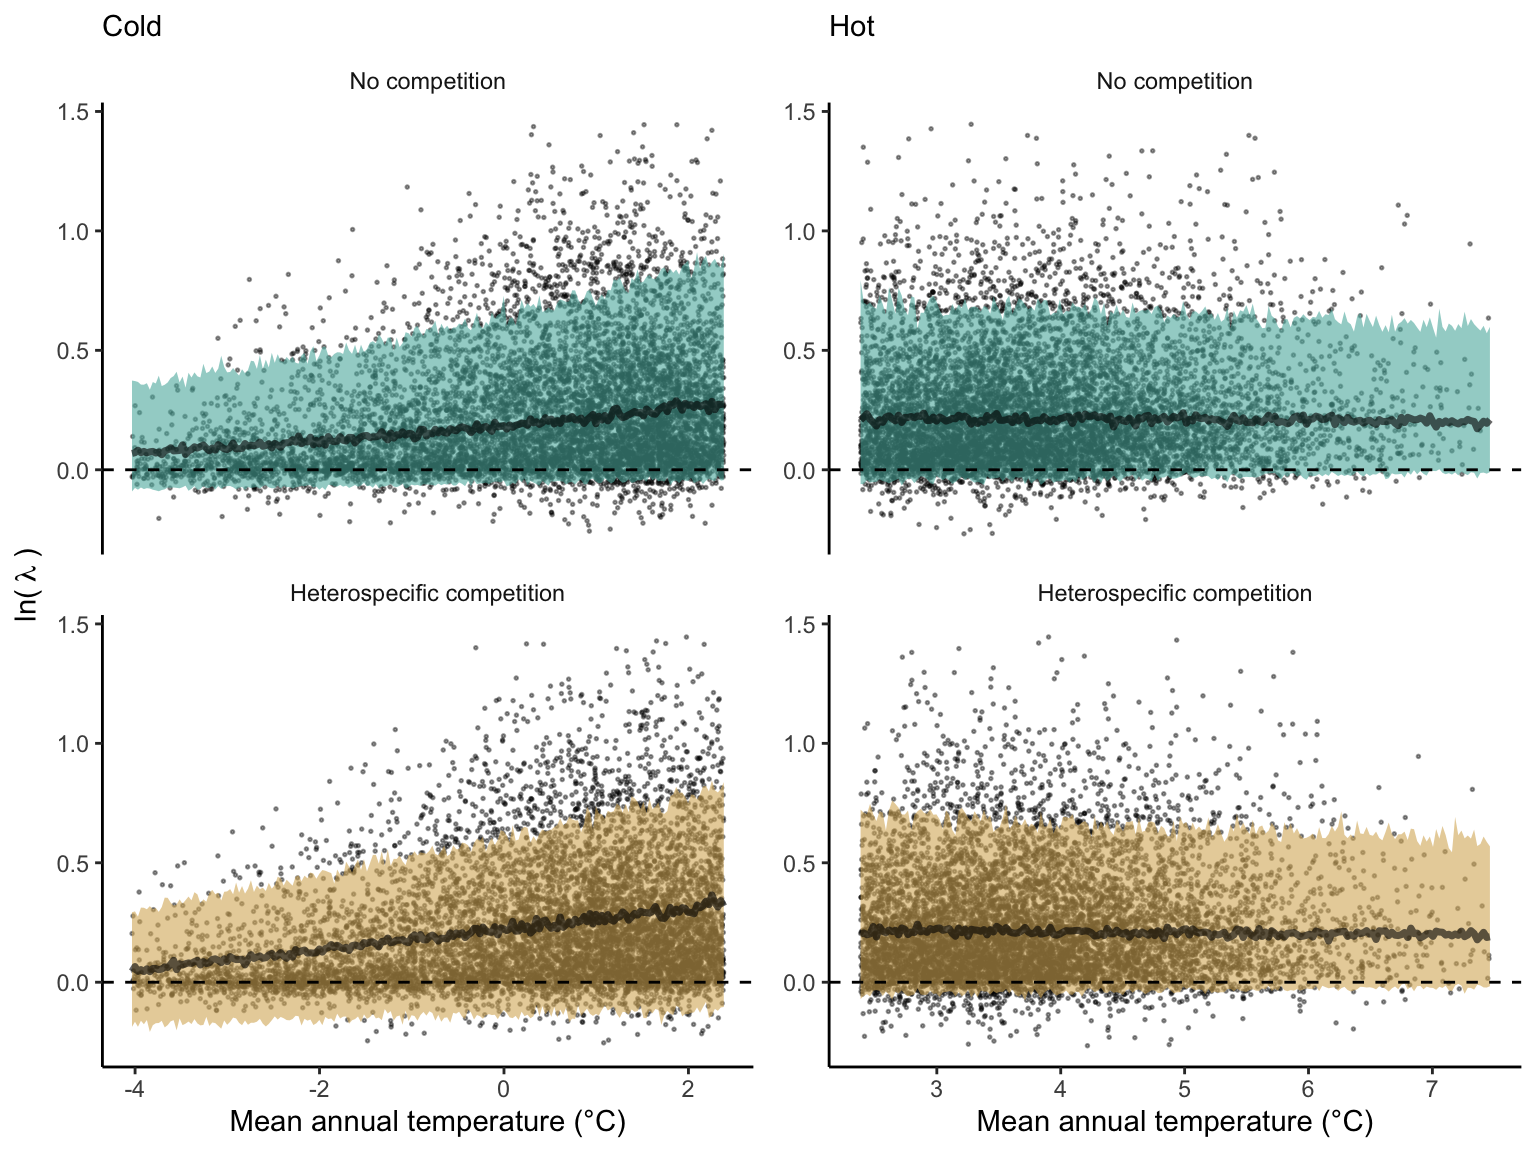
\includegraphics[width=1\textwidth,height=\textheight]{https://willvieira.github.io/book_forest-demography-IPM/extinction_risk_files/figure-html/fig-res_example-1.png}
\caption{Distribution of stochastic population growth rate (\(\lambda\))
for \emph{Abies balsamea} over the mean annual temperature gradient for
cold (left panels) and hot (right panels) ranges under no competition
(fundamental niche) and heterospecific competition (realized niche). The
dots represent \(\lambda\) over the plot-year-replication combinations.
The model's average line and 90\% prediction intervals are estimated
using 500 draws from the posterior distribution.}\label{fig:res_example}
}
\end{figure}

We then investigated the local suitability probability using the
empirical cumulative distribution approach (Equation \ref{eq:sp}) from
the linear model predictions. The Figure \ref{fig:sp-example} shows the
suitable probability expected over the mean annual temperature of the
same species. We observed that the local suitability probability was
reduced towards the cold border, with a stronger reduction under
heterospecific competition (yellow curve). We can also observe that the
decrease in suitable probability towards the border is nonlinear,
becoming more substantial for heterospecific competition than for the
no-competition condition.

The model fit and the estimation of suitable probability across the
temperature gradient for all species are presented in Supplementary
Material 2. We observed for most species a decrease of the climate
effect at one border while the other remained unchanged. Additionally, a
few species displayed a clear linear pattern of decreasing suitable
probability from the cold to the hot border, with only one species
(\emph{Betula papyrifera}) having a decrease at both borders.
Conversely, under the competition effect, most species exhibited a
decrease in suitable probability at the hot border and an increase at
the cold border, indicating a linear rise in the impact of competition
from the cold to the hot border of the distribution.

\begin{figure}
\hypertarget{fig:sp-example}{%
\centering
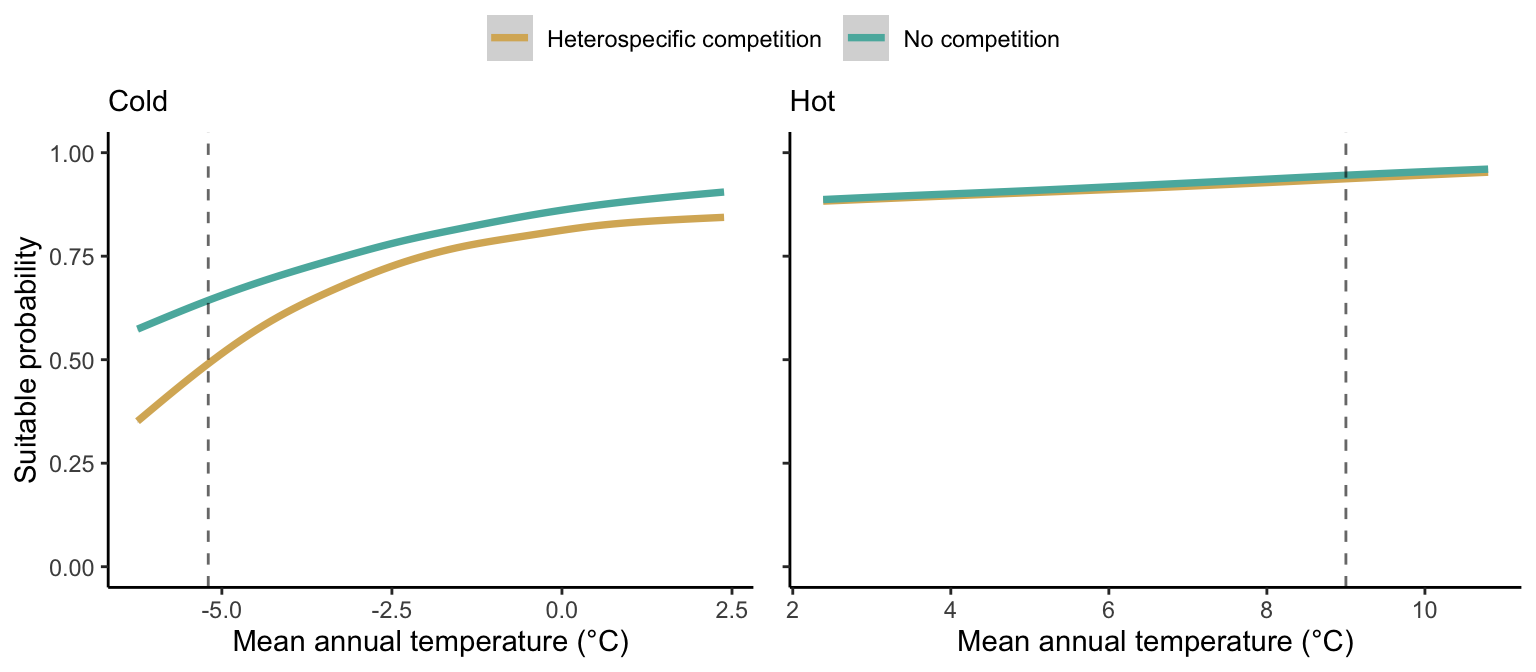
\includegraphics[width=1\textwidth,height=\textheight]{https://willvieira.github.io/book_forest-demography-IPM/extinction_risk_files/figure-html/fig-sp-example-1.png}
\caption{Suitable probability of \emph{Abies balsamea} over the mean
annual temperature gradient for cold and hot ranges under no competition
(green) and heterospecific (yellow). The vertical dotted line represents
the range limits of the MAT observed in the
dataset.}\label{fig:sp-example}
}
\end{figure}

\hypertarget{effect-of-climate-and-competition-on-suitable-probability-for-the-center-and-border-distributions}{%
\subsubsection{Effect of climate and competition on suitable probability
for the center and border
distributions}\label{effect-of-climate-and-competition-on-suitable-probability-for-the-center-and-border-distributions}}

We investigated the effect of climate and competition on the suitable
probability at the border and center of the temperature range
distribution for all species. Because the border and center positions
are relative to each species, we could not represent the continuous
trend in suitable probability across the MAT for all 31 species
together. Instead, we extracted the local suitable probability with and
without heterospecific competition for four locations across the MAT
gradient (Figure \ref{fig:sp_comp_vs_nocomp2}). Overall, suitable
probability was high among the species, with an average of 0.78. Among
the four locations, species presented a lower suitable probability at
the border of the hot range, with an average of 0.67. Across the
temperature range, there is a monotonic decrease in suitable probability
from the cold border toward the hot border.

\begin{figure}
\hypertarget{fig:sp_comp_vs_nocomp2}{%
\centering
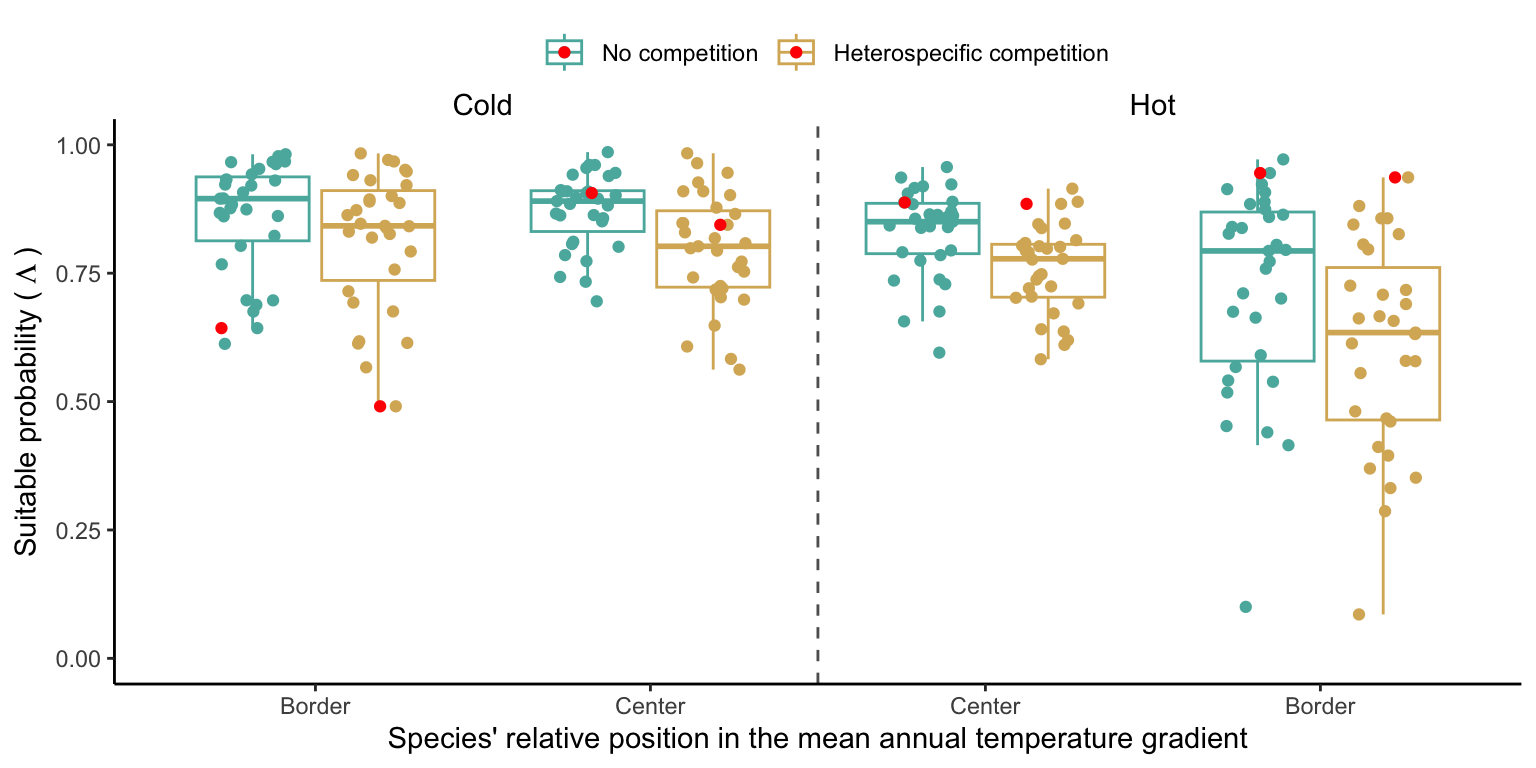
\includegraphics[width=1\textwidth,height=\textheight]{https://willvieira.github.io/book_forest-demography-IPM/extinction_risk_files/figure-html/fig-sp_comp_vs_nocomp2-1.png}
\caption{Estimated suitable probability for the 31 forest species across
across the center and border of the cold and hot ranges. The x-axis
represents the mean annual temperature gradient similar to Figure
\ref{fig:sp-example}, but is discretized at the border and center limits
relative to each species. We highlighted the balsam fir species in red.
Note that we omitted the parameter uncertainty of each species in this
figure to avoid overlap and increase
clarity.}\label{fig:sp_comp_vs_nocomp2}
}
\end{figure}

We further disentangle the influence of competition from that of climate
by calculating the difference between suitable probability under
heterospecific competition and without competition. A negative
difference signifies competition reduces suitable probability, while
positive differences indicate an increase. Across the four climate
locations, heterospecific competition consistently reduced suitable
probability for most species, with the magnitude of reduction
intensifying from the cold to the hot border (Figure S1). This suggests
that the decline in suitable probability observed from the cold to the
hot border (Figure \ref{fig:sp_comp_vs_nocomp2}) results from the
combined effect of climate and competition.

\hypertarget{suitable-probability-change-from-center-to-border}{%
\subsubsection{Suitable probability change from center to
border}\label{suitable-probability-change-from-center-to-border}}

We investigated the relative effect of climate and competition on
changing suitable probability from the center to the border of the
species distribution (Figure \ref{fig:diff_sp_hist}). A positive
relative difference indicates an increase in suitable probability from
the center towards the border, while a negative difference indicates a
decrease. Most species exhibited a decrease in suitable probability at
the hot border relative to the center. Alternatively, most species
showed a reduction in the effect of competition toward the cold border.
However, the climate effect in the cold range was more variable, with
some species experiencing an increase and others a decrease in suitable
probability. Overall, the relative difference in suitable probability
from the center toward the cold and hot borders was more influenced by
climate rather than competition.

\begin{figure}
\hypertarget{fig:diff_sp_hist}{%
\centering
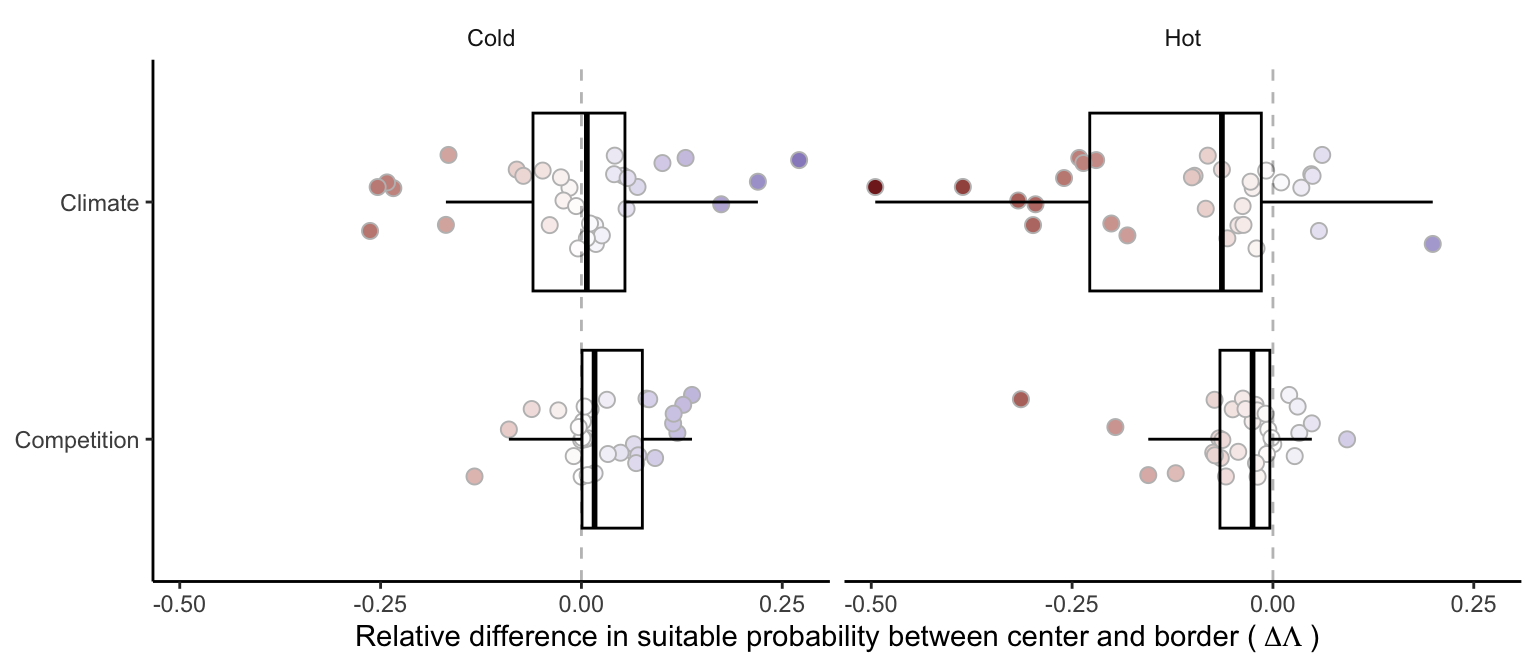
\includegraphics[width=1\textwidth,height=\textheight]{https://willvieira.github.io/book_forest-demography-IPM/extinction_risk_files/figure-html/fig-diff_sp_hist-1.png}
\caption{Difference in suitable probability for climate and competition
effects over the cold and hot ranges. Negative values denote a decrease
in species suitable probability from the center towards the distribution
border, while positive values indicate an increase. Specifically, a
negative value for climate at the hot (or cold) range signifies a
reduction in suitable probability as temperature rises (or falls)
towards the border. Boxplots determine the 25-75 quantile distribution
among the species.}\label{fig:diff_sp_hist}
}
\end{figure}

\hypertarget{discussion}{%
\section{Discussion}\label{discussion}}

Understanding the mechanisms shaping species distribution is imperative
to face ongoing global changes. We acknowledged and integrated various
sources of variability in the population growth rate of forest trees,
contributing to an improved understanding of forest dynamics in an
uncertain world. Introducing a novel metric, we quantified the relative
impacts of climate and competition on the change in suitable probability
across species distributions. Our findings revealed a nearly linear
reduction in suitable probability from the cold to hot borders. Notably,
the predominant influence on the relative difference in suitable
probability from the center toward the border was attributed to climate
rather than competition. These results, supported by a novel approach
accounting for uncertainty, enhance our understanding of the nuanced
interplay between climate and competition across species ranges.

The suitable probability was high across all species and range
locations, with only around 5\% of all species-location combinations
having a suitable probability below the 0.5 threshold. This is primarily
attributed to most species exhibiting a high positive population growth
rate across their current range distribution. Additionally, the
spatio-temporal variability in the environment and the parameter
uncertainty in the plot may contribute to the elevated average
population growth rate due to nonlinear averaging. This aligns with
theoretical (Schreiber and Lloyd-Smith
\protect\hyperlink{ref-Schreiber2009}{2009}) and empirical (Crone
\protect\hyperlink{ref-Crone2016}{2016}) studies suggesting that spatial
heterogeneity should increase the population growth rate.

Competition significantly reduces local suitability across all range
locations, with a stronger and more consistent effect at the cold
border, contributing to the ongoing debate surrounding its significance
in setting range limits. Despite several studies emphasizing the effect
of competition compared to climate on the demographic rates of forest
trees (Zhang et al. \protect\hyperlink{ref-Zhang2015}{2015}, Käber et
al. \protect\hyperlink{ref-Kaber2021}{2021}, Le Squin et al.
\protect\hyperlink{ref-LeSquin2021}{2021}), debates persist regarding
whether this effect at the local scale translates to the biogeographic
distribution of species (Sober\a'on
\protect\hyperlink{ref-Soberon2007}{2007}, Copenhaver-Parry et al.
\protect\hyperlink{ref-CopenhaverParry2017}{2017}). Our findings support
the Godsoe et al. (\protect\hyperlink{ref-Godsoe2017}{2017}) hypothesis
and a growing body of evidence (Scherrer et al.
\protect\hyperlink{ref-Scherrer2020}{2020}, Shi et al.
\protect\hyperlink{ref-Shi2020}{2020}, Paquette and Hargreaves
\protect\hyperlink{ref-Paquette2021}{2021}, Lyu and Alexander
\protect\hyperlink{ref-Lyu2022}{2022}) showing that the effect of
competition on the intrinsic population growth rate can indeed
contribute to range limits.

The decline in suitable probability from the cold to the hot border
suggests a predominantly linear, rather than unimodal, relationship with
temperature for most species. This result is consistent with reduced
population growth rates in North American (Le Squin et al.
\protect\hyperlink{ref-LeSquin2021}{2021}, Schultz et al.
\protect\hyperlink{ref-schultz2022}{2022}) and European (Guyennon et al.
\protect\hyperlink{ref-Guyennon2023}{2023}) forest trees, except for the
contrasting pattern observation by Purves
(\protect\hyperlink{ref-Purves2009}{2009}). The higher suitable
probability in the cold range compared to the hot range could be
attributed to multiple factors. First, species may still follow their
climate niche post the last glaciation, explaining why the current cold
range limit does not align with the expected niche distribution
(Svenning and Skov \protect\hyperlink{ref-Svenning2007}{2007}),
potentially leading to a colonization debt (Talluto et al.
\protect\hyperlink{ref-Talluto2017}{2017}). Notably, four of the six
species exhibiting a significant decrease in suitable probability from
the center toward the cold range were already at the extreme cold
observed in the dataset (Figure S4).

Our model may however overlook crucial drivers of species performance,
despite capturing a substantial amount of variation from parameter
uncertainty at the plot level. Factors such as the impact of extreme
temperature and precipitation on phenology can influence tree range
limits (Morin et al. \protect\hyperlink{ref-Morin2007}{2007}). Beyond
covariates and plot-level uncertainty, incorporating temporal
uncertainty at the plot level, accounting for spatio-temporal
covariance, could likely capture additional sources of variation in
demographic rates. While our approach considers temporal stochasticity
in climate and competition, which affect species range size (Holt et al.
\protect\hyperlink{ref-Holt2022}{2022}), there remains temporal
variation in demographic rates beyond these covariates. This
variability, possibly captured with random effects at the plot level,
can influence range limits based on the degree of temporal
autocorrelation and its relationship with the range (Benning et al.
\protect\hyperlink{ref-Benning2022}{2022}). For instance, an empirical
study on perennial herbaceous species demonstrated that temporal
environmental stochasticity reduced the population growth rate relative
to the average (Crone \protect\hyperlink{ref-Crone2016}{2016}). In our
study, this temporal variability is particularly relevant for survival
(due to disturbance) and recruitment (due to phenology) rates because,
in addition to having high temporal variability (Clark et al.
\protect\hyperlink{ref-Clark1999a}{1999}, de Souza Leite et al.
\protect\hyperlink{ref-Leite2023}{2023}), they represent the most
significant drivers of population growth rate (Chapter 2).

The effect of competition, similar to climate, increased from the center
towards the border of the hot range, contrary to Kunstler et al.
(\protect\hyperlink{ref-Kunstler2021}{2021}), who found no difference in
the competition effect between the center and border of the species.
Additionally, our results deviate from the Species Interactions-Abiotic
Stress Hypothesis, predicting a stronger competition effect in less
stressful climate conditions (Louthan et al.
\protect\hyperlink{ref-Louthan2015}{2015}). When considering the
relative position of the species across the temperature gradient, only
the effect of climate at the cold range changed with temperature. This
indicates that most species have a similar or higher suitable
probability at the border of the cold range compared to their center
distribution. We further tested whether the species' range size affects
the relative difference in suitable probability; while the absolute
values change, the pattern among the species remains unchanged.

The climate gradient of temperature had a more significant effect than
competition in changing the suitable probability of forest trees. This
means that mean annual temperature, along with all latent variables,
better explains how suitable probability changes across the temperature
range. The choice of using only mean annual temperature as an
explanatory variable for the variance of \(\lambda\) can be improved.
For instance, the model could be built accounting for mean annual
temperature and precipitation to predict the complete two-dimensional
distribution of the species' climate niche. Plot random effects could be
further used to account for the nestedness of the data design, allowing
the proper separation of the total variance of the metamodel into
variance arising from individual- and plot-level demographic
uncertainty. While we have assumed climate variability as independent
and identically distributed random variables, this assumption can be
relaxed to include temporal autocorrelation. Autocorrelated
environmental fluctuation can significantly change a species' range
limits due to nonlinear averaging (Benning et al.
\protect\hyperlink{ref-Benning2022}{2022}, Holt et al.
\protect\hyperlink{ref-Holt2022}{2022}). Lastly, although coexistence
theory assumes the abundance of competitors to be at equilibrium
(Chesson \protect\hyperlink{ref-Chesson2000a}{2000}), testing this
assumption remains practically impossible.

Despite the many ways of improving our study, there is a growing body of
evidence indicating a mismatch between performance and occurrence
(McGill \protect\hyperlink{ref-McGill2012}{2012}, Csergo et al.
\protect\hyperlink{ref-Csergo2017}{2017}, Bohner and Diez
\protect\hyperlink{ref-bohner2020}{2020}, Le Squin et al.
\protect\hyperlink{ref-LeSquin2021}{2021}, Midolo et al.
\protect\hyperlink{ref-Midolo2021}{2021}, Guyennon et al.
\protect\hyperlink{ref-Guyennon2023}{2023}, Thuiller et al.
\protect\hyperlink{ref-Thuiller2014}{2014}). Our approach can better
capture the nuanced effect of climate and competition along with the
spatio-temporal variation in \(\lambda\), yet it was not enough to fully
predict tree range limits. Since species distribution is influenced by
processes at multiple scales (McGill
\protect\hyperlink{ref-McGill2010}{2010}, Heffernan et al.
\protect\hyperlink{ref-Heffernan2014}{2014}), it is challenging to rely
on a single individual-level performance metric to predict it all (Evans
et al. \protect\hyperlink{ref-Evans2016}{2016}). For instance,
dispersion plays a crucial role in changing species distribution at
larger spatial scales, either reducing its extent due to limited
dispersal or increasing it through source-sink dynamics (Pulliam
\protect\hyperlink{ref-Pulliam2000}{2000}). We propose that our novel
metric, local suitable probability, can be a key unifying factor linking
local and landscape scales.

Forest trees exhibit variation in their frequency of occurrence across
distribution gradients, yet their relative abundance remains consistent
when present (Canham and Thomas
\protect\hyperlink{ref-Canham2010}{2010}). Such observation implies that
assessing forest distribution should focus on colonization and
extinction patch dynamics rather than local performance (Canham and
Murphy \protect\hyperlink{ref-Canham2017}{2017}). However, instead of
restricting models to either local or large scales, we propose using the
local suitable probability to reconcile the local demographic dynamics
with the metapopulation theory. Colonization and extinction processes,
as described by metapopulation theory (Levins
\protect\hyperlink{ref-Levins1969}{1969}), are well-suited for
describing the mosaic of forest successional stages at the landscape
scale resulting from natural disturbances and succession. However, an
implicit assumption is that unoccupied patches are necessarily available
for colonization. We relax this assumption and quantify patch
availability using the local suitable probability metric (\(\Lambda\)).
Take an ensable of patches (\(p\)) where individuals can arrive and
establish empty patches through colonization (\(\alpha\)), and occupied
patches can become empty through extinction (\(\varepsilon\)):
Considering an ensemble of patches (\(p\)) where individuals can arrive
and establish in empty patches through colonization (\(\alpha\)), and
occupied patches can become empty through extinction (\(\varepsilon\)),
the integrated metapopulation model becomes:

\[
\frac{dp}{dt} = \alpha p (\Lambda - p) - \varepsilon p
\]

With this formulation, rather than having \(1 - p\) available patches
for colonization, we have \(\Lambda - p\). Therefore, when \(\lambda\)
and its variability are high, the local suitable probability equals 1,
indicating that all non-occupied patches are available. Conversely, as
the local suitable probability decreases, the proportion of non-occupied
patches available for colonization is reduced. This integrative approach
allows one to account for both the local (e.g.~competition and climate)
and landscape (e.g.~fire disturbances and dispersal) drivers of forest
dynamics when assessing tree distribution.

\hypertarget{references}{%
\section*{References}\label{references}}
\addcontentsline{toc}{section}{References}

\hypertarget{refs}{}
\begin{cslreferences}
\leavevmode\hypertarget{ref-Benning2022}{}%
Benning, J. W., R. A. Hufbauer, and C. Weiss-Lehman. 2022. Increasing
temporal variance leads to stable species range limits. Proceedings of
the Royal Society B: Biological Sciences 289.

\leavevmode\hypertarget{ref-bohner2020}{}%
Bohner, T., and J. Diez. 2020. Extensive mismatches between species
distributions and performance and their relationship to functional
traits. Ecology Letters 23:33--44.

\leavevmode\hypertarget{ref-Canham2017}{}%
Canham, C. D., and L. Murphy. 2017. The demography of tree species
response to climate: Sapling and canopy tree survival. Ecosphere 8.

\leavevmode\hypertarget{ref-Canham2010}{}%
Canham, C. D., and R. Q. Thomas. 2010. Frequncy, not relative abundance,
of temperate tree species varies along climate gradients in eastern
North America. Ecology 91:3433--3440.

\leavevmode\hypertarget{ref-Caswell2009}{}%
Caswell, H. 2009. Stage, age and individual stochasticity in demography.
Oikos 118:1763--1782.

\leavevmode\hypertarget{ref-Chesson2000a}{}%
Chesson, P. 2000. Mechanisms of maintenance of species diversity. Annu.
Rev. Ecol. Syst 31:343--66.

\leavevmode\hypertarget{ref-Clark2010}{}%
Clark, J. S. 2010. Individuals and the variation needed for high species
diversity in forest trees. Science 327:1129--1132.

\leavevmode\hypertarget{ref-Clark1999a}{}%
Clark, J. S., B. Beckage, P. Camill, B. Cleveland, J. HilleRisLambers,
J. Lichter, J. McLachlan, J. Mohan, and P. Wyckoff. 1999. Interpreting
recruitment limitation in forests. American Journal of Botany 86:1--16.

\leavevmode\hypertarget{ref-CopenhaverParry2017}{}%
Copenhaver-Parry, P. E., B. N. Shuman, and D. B. Tinker. 2017. Toward an
improved conceptual understanding of North American tree species
distributions. Ecosphere 8:e01853.

\leavevmode\hypertarget{ref-Cressie2009}{}%
Cressie, N., C. A. Calder, J. S. Clark, J. M. Ver Hoef, and C. K. Wikle.
2009. Accounting for uncertainty in ecological analysis: The strengths
and limitations of hierarchical statistical modeling. Ecological
Applications 19:553--570.

\leavevmode\hypertarget{ref-Crone2016}{}%
Crone, E. E. 2016. Contrasting effects of spatial heterogeneity and
environmental stochasticity on population dynamics of a perennial
wildflower. Journal of Ecology 104:281--291.

\leavevmode\hypertarget{ref-Csergo2017}{}%
Csergo, A. M., R. Salguero-G\a'omez, O. Broennimann, S. R. Coutts, A.
Guisan, A. L. Angert, E. Welk, I. Stott, B. J. Enquist, B. McGill, J.-C.
Svenning, C. Violle, and Y. M. Buckley. 2017. Less favourable climates
constrain demographic strategies in plants. Ecology Letters.

\leavevmode\hypertarget{ref-Damgaard2020}{}%
Damgaard, C. 2020. Measurement Uncertainty in Ecological and
Environmental Models. Trends in Ecology and Evolution 35:871--873.

\leavevmode\hypertarget{ref-Leite2023}{}%
de Souza Leite, M., S. M. McMahon, P. I. Prado, S. J. Davies, A. A. de
Oliveira, H. P. D. Deurwaerder, S. Aguilar, K. J. Anderson-Teixeira, N.
Aqilah, N. A. Bourg, W. Y. Brockelman, N. Castaño, C.-H. Chang-Yang,
Y.-Y. Chen, G. Chuyong, K. Clay, \a'Alvaro Duque, S. Ediriweera, C. E.
N. Ewango, G. Gilbert, I. A. U. N. Gunatilleke, C. V. S. Gunatilleke, R.
Howe, W. H. Huasco, A. Itoh, D. J. Johnson, D. Kenfack, K. Kr\a'al, Y.
T. Leong, J. A. Lutz, J.-R. Makana, Y. Malhi, W. J. McShea, M. Mohamad,
M. Nasardin, A. Nathalang, G. Parker, R. Parmigiani, R. P\a'erez, R. P.
Phillips, P. Šamonil, I.-F. Sun, S. Tan, D. Thomas, J. Thompson, M.
Uriarte, A. Wolf, J. Zimmerman, D. Zuleta, M. D. Visser, and L.
Hülsmann. 2023. Major axes of variation in tree demography across global
forests. bioRxiv.

\leavevmode\hypertarget{ref-Ellner2016}{}%
Ellner, S. P., D. Z. Childs, and M. Rees. 2016. Data-driven modelling of
structured populations. Springer.

\leavevmode\hypertarget{ref-Ettinger2017}{}%
Ettinger, A., and J. HilleRisLambers. 2017. Competition and facilitation
may lead to asymmetric range shift dynamics with climate change. Global
Change Biology 23:3921--3933.

\leavevmode\hypertarget{ref-Evans2016}{}%
Evans, M. E. K., C. Merow, S. Record, S. M. McMahon, and B. J. Enquist.
2016. Towards Process-based Range Modeling of Many Species. Trends in
Ecology and Evolution 31:860--871.

\leavevmode\hypertarget{ref-cmdstanr}{}%
Gabry, J., R. Češnovar, and A. Johnson. 2023. cmdstanr: R Interface to
'CmdStan'.

\leavevmode\hypertarget{ref-Godsoe2017}{}%
Godsoe, W., J. Jankowski, R. D. Holt, and D. Gravel. 2017. Integrating
Biogeography with Contemporary Niche Theory. Trends in Ecology and
Evolution 32:488--499.

\leavevmode\hypertarget{ref-Gravel2011}{}%
Gravel, D., F. Guichard, and M. E. Hochberg. 2011. Species coexistence
in a variable world. Ecology Letters 14:828--839.

\leavevmode\hypertarget{ref-Guyennon2023}{}%
Guyennon, A., B. Reineking, R. Salguero-Gomez, J. Dahlgren, A. Lehtonen,
S. Ratcliffe, P. Ruiz-Benito, M. A. Zavala, and G. Kunstler. 2023.
Beyond mean fitness: Demographic stochasticity and resilience matter at
tree species climatic edges. Global Ecology and Biogeography
32:573--585.

\leavevmode\hypertarget{ref-Harwood2003}{}%
Harwood, J., and K. Stokes. 2003. Coping with uncertainty in ecological
advice: Lessons from fisheries. Trends in Ecology and Evolution
18:617--622.

\leavevmode\hypertarget{ref-Heffernan2014}{}%
Heffernan, J. B., P. A. Soranno, M. J. Angilletta, L. B. Buckley, D. S.
Gruner, T. H. Keitt, J. R. Kellner, J. S. Kominoski, A. V. Rocha, and J.
Xiao. 2014. Macrosystems ecology: understanding ecological patterns and
processes at continental scales. Frontiers in Ecology and the
Environment 12:5--14.

\leavevmode\hypertarget{ref-holt2009}{}%
Holt, R. D. 2009. Bringing the Hutchinsonian niche into the 21st
century: ecological and evolutionary perspectives. Proceedings of the
National Academy of Sciences 106:19659--19665.

\leavevmode\hypertarget{ref-Holt2022}{}%
Holt, R. D., M. Barfield, and J. H. Peniston. 2022. Temporal variation
may have diverse impacts on range limits. Philosophical Transactions of
the Royal Society B: Biological Sciences 377.

\leavevmode\hypertarget{ref-Holt2005}{}%
Holt, R. D., T. H. Keitt, M. a Lewis, B. a Maurer, and M. L. Taper.
2005. Theoretical models of species' borders: single species approaches.
Schurr2012 108:18--27.

\leavevmode\hypertarget{ref-Hutchinson1957}{}%
Hutchinson, G. E. 1957. Concluding remarks. Pages 415--427 \emph{in}
Cold spring harbor symposium on quantitative biology.

\leavevmode\hypertarget{ref-Kaber2021}{}%
Käber, Y., P. Meyer, J. Stillhard, E. De Lombaerde, J. Zell, G.
Stadelmann, H. Bugmann, and C. Bigler. 2021. Tree recruitment is
determined by stand structure and shade tolerance with uncertain role of
climate and water relations. Ecology and Evolution 11:12182--12203.

\leavevmode\hypertarget{ref-Koons2009}{}%
Koons, D. N., S. Pavard, A. Baudisch, and C. Jessica E. Metcalf. 2009.
Is life-history buffering or lability adaptive in stochastic
environments? Oikos 118:972--980.

\leavevmode\hypertarget{ref-Kunstler2021}{}%
Kunstler, G., A. Guyennon, S. Ratcliffe, N. Rüger, P. Ruiz-Benito, D. Z.
Childs, J. Dahlgren, A. Lehtonen, W. Thuiller, C. Wirth, M. A. Zavala,
and R. Salguero-Gomez. 2021. Demographic performance of European tree
species at their hot and cold climatic edges. Journal of Ecology
109:1041--1054.

\leavevmode\hypertarget{ref-leslie1945}{}%
Leslie, P. H. 1945. On the use of matrices in certain population
mathematics. Sankhyt 33:183--212.

\leavevmode\hypertarget{ref-LeSquin2021}{}%
Le Squin, A., I. Boulangeat, and D. Gravel. 2021. Climate-induced
variation in the demography of 14 tree species is not sufficient to
explain their distribution in eastern North America. Global Ecology and
Biogeography 30:352--369.

\leavevmode\hypertarget{ref-Levins1969}{}%
Levins, R. 1969. Some Demographic and Genetic Consequences of
Environmental Heterogeneity for Biological Control. Bulletin of the
Entomological Society of America 15:237--240.

\leavevmode\hypertarget{ref-Lewis1942}{}%
Lewis, E. G. 1942. On the generation and growth of a population. Sankhyã
6:93--96.

\leavevmode\hypertarget{ref-Louthan2015}{}%
Louthan, A. M., D. F. Doak, and A. L. Angert. 2015. Where and When do
Species Interactions Set Range Limits? Trends in Ecology and Evolution
30:780--792.

\leavevmode\hypertarget{ref-Lyu2022}{}%
Lyu, S., and J. M. Alexander. 2022. Competition contributes to both warm
and cool range edges. Nature Communications 13:1--9.

\leavevmode\hypertarget{ref-maguire1973niche}{}%
Maguire Jr, B. 1973. Niche response structure and the analytical
potentials of its relationship to the habitat. The American Naturalist
107:213--246.

\leavevmode\hypertarget{ref-May1978}{}%
May, R. M., J. R. Beddington, J. W. Horwood, and J. G. Shepherd. 1978.
Exploiting natural populations in an uncertain world. Mathematical
Biosciences 42:219--252.

\leavevmode\hypertarget{ref-McGill2010}{}%
McGill, B. J. 2010. Matters of scale. Science 328:575--576.

\leavevmode\hypertarget{ref-McGill2012}{}%
McGill, B. J. 2012. Trees are rarely most abundant where they grow best.
Journal of Plant Ecology 5:46--51.

\leavevmode\hypertarget{ref-Midolo2021}{}%
Midolo, G., C. Wellstein, and S. Faurby. 2021. Individual fitness is
decoupled from coarse-scale probability of occurrence in North American
trees. Ecography 44:789--801.

\leavevmode\hypertarget{ref-milles2023}{}%
Milles, A., T. Banitz, M. Bielcik, K. Frank, C. A. Gallagher, F.
Jeltsch, J. U. Jepsen, D. Oro, V. Radchuk, and V. Grimm. 2023. Local
buffer mechanisms for population persistence. Trends in Ecology \&
Evolution 38:1051--1059.

\leavevmode\hypertarget{ref-Naturelles2016}{}%
Ministere des Ressources Naturelles. 2016. Norme d'inventaire
ecoforestier: placettes-echantillons temporaires. Direction des
inventaires forestier, Ministère des Ressources naturelles,Québec.

\leavevmode\hypertarget{ref-Morin2007}{}%
Morin, X., C. Augspurger, and I. Chuine. 2007. Process-based modeling of
species' distributions: what limits temperate tree species' range
boundaries? Ecology 88:2280--2291.

\leavevmode\hypertarget{ref-OConnell2007}{}%
O'Connell, M. B., E. B. LaPoint, J. A. Turner, T. Ridley, D. Boyer, A.
Wilson, K. L. Waddell, and B. L. Conkling. 2007. The forest inventory
and analysis database: Database description and users forest inventory
and analysis program. US Department of Agriculture, Forest Service.

\leavevmode\hypertarget{ref-Paquette2021}{}%
Paquette, A., and A. L. Hargreaves. 2021. Biotic interactions are more
often important at species' warm versus cool range edges. Ecology
Letters 24:2427--2438.

\leavevmode\hypertarget{ref-Pulliam2000}{}%
Pulliam, H. R. 2000. On the relationship between niche and distribution.
Ecology Letters 3:349--361.

\leavevmode\hypertarget{ref-Purves2009}{}%
Purves, D. W. 2009. The demography of range boundaries versus range
cores in eastern US tree species. Proceedings of the Royal Society B:
Biological Sciences 276:1477--1484.

\leavevmode\hypertarget{ref-Scherrer2020}{}%
Scherrer, D., Y. Vitasse, A. Guisan, T. Wohlgemuth, and H. Lischke.
2020. Competition and demography rather than dispersal limitation slow
down upward shifts of trees' upper elevation limits in the Alps. Journal
of Ecology:1--15.

\leavevmode\hypertarget{ref-Schreiber2009}{}%
Schreiber, S. J., and J. O. Lloyd-Smith. 2009. Invasion dynamics in
spatially heterogeneous environments. American Naturalist 174:490--505.

\leavevmode\hypertarget{ref-schultz2022}{}%
Schultz, E. L., L. Hülsmann, M. D. Pillet, F. Hartig, D. D. Breshears,
S. Record, J. D. Shaw, R. J. DeRose, P. A. Zuidema, and M. E. K. Evans.
2022. Climate-driven, but dynamic and complex? A reconciliation of
competing hypotheses for species' distributions. Ecology letters
25:38--51.

\leavevmode\hypertarget{ref-Shi2020}{}%
Shi, H., Q. Zhou, F. Xie, N. He, R. He, K. Zhang, Q. Zhang, and H. Dang.
2020. Disparity in elevational shifts of upper species limits in
response to recent climate warming in the Qinling Mountains,
North-central China. Science of the Total Environment 706:135718.

\leavevmode\hypertarget{ref-Shoemaker2020}{}%
Shoemaker, L. G., L. L. Sullivan, I. Donohue, J. S. Cabral, R. J.
Williams, M. M. Mayfield, J. M. Chase, C. Chu, W. S. Harpole, A. Huth,
J. HilleRisLambers, A. R. M. James, N. J. B. Kraft, F. May, R.
Muthukrishnan, S. Satterlee, F. Taubert, X. Wang, T. Wiegand, Q. Yang,
and K. C. Abbott. 2020. Integrating the underlying structure of
stochasticity into community ecology. Ecology 101:1--15.

\leavevmode\hypertarget{ref-Sittaro2017}{}%
Sittaro, F., A. Paquette, C. Messier, and C. A. Nock. 2017. Tree range
expansion in eastern North America fails to keep pace with climate
warming at northern range limits. Global Change Biology:1--10.

\leavevmode\hypertarget{ref-Soberon2007}{}%
Sober\a'on, J. 2007. Grinnellian and Eltonian niches and geographic
distributions of species. Ecology Letters 10:1115--1123.

\leavevmode\hypertarget{ref-Svenning2007}{}%
Svenning, J. C., and F. Skov. 2007. Could the tree diversity pattern in
Europe be generated by postglacial dispersal limitation? Ecology Letters
10:453--460.

\leavevmode\hypertarget{ref-Talluto2017}{}%
Talluto, M. V., I. Boulangeat, S. Vissault, W. Thuiller, and D. Gravel.
2017. Extinction debt and colonization credit delay range shifts of
eastern North American trees. Nature Ecology \& Evolution 1:0182.

\leavevmode\hypertarget{ref-stan2022stan}{}%
Team, S. D., and Others. 2022. Stan modeling language users guide and
reference manual, version 2.30.1. Stan Development Team.

\leavevmode\hypertarget{ref-Terry2022}{}%
Terry, J. C. D., J. D. O'Sullivan, and A. G. Rossberg. 2022.
Synthesising the multiple impacts of climatic variability on community
responses to climate change. Ecography 2022:e06123.

\leavevmode\hypertarget{ref-Thuiller2014}{}%
Thuiller, W., T. Munkemuller, K. H. Schiffers, D. Georges, S. Dullinger,
V. M. Eckhart, T. C. Edwards, D. Gravel, G. Kunstler, C. Merow, K.
Moore, C. Piedallu, S. Vissault, N. E. Zimmermann, D. Zurell, F. M.
Schurr, T. Münkemüller, K. H. Schiffers, D. Georges, S. Dullinger, V. M.
Eckhart, T. C. Edwards, D. Gravel, G. Kunstler, C. Merow, K. Moore, C.
Piedallu, S. Vissault, N. E. Zimmermann, D. Zurell, and F. M. Schurr.
2014. Does probability of occurrence relate to population dynamics?
Ecography 37:1155--1166.

\leavevmode\hypertarget{ref-van2020}{}%
van Daalen, S., and H. Caswell. 2020. Variance as a life history
outcome: Sensitivity analysis of the contributions of stochasticity and
heterogeneity. Ecological Modelling 417.

\leavevmode\hypertarget{ref-Zhang2015}{}%
Zhang, J., S. Huang, and F. He. 2015. Half-century evidence from western
Canada shows forest dynamics are primarily driven by competition
followed by climate. Proceedings of the National Academy of Sciences
112:4009--4014.
\end{cslreferences}


\newpage


\end{document}